% Векторизация метода погруженных границ - потери производительности при векторизаии неплоских циклов.
\subsection{Векторизация с помощью представления расчетов в виде композиции плоских циклов}

В том случае, если вычисления организованы таким образом, что они могут трактоваться как композиция плоских циклов, а тела этих плоских циклов являются достаточно простыми с точки зрения управления, оптимизирующий компилятор может успешно создавать векторизованный код.
В этом случае даже нет необходимости явно использовать ассемблерные вставки или функции-интринсики.
В данном разделе рассмотрим основные аспекты приведения программного кода в форму, пригодную для автоматической векторизации \cite{Rybakov2023VecIBM}.
Подходы, применяемые к векторизации плоских циклов, могут применяться также к циклам, которые не являются плоскими.
Такие циклы все равно могут быть векторизованы, однако это может приводить к потере производительности.
Также в этом разделе будет проведен анализ потерь производительности при отклонении от свойств плоских циклов на примере газодинамических расчетов с использованием метода погруженных границ для расчета обтекания тела со сложной геометрией.

\subsubsection{Постановка задачи газовой динамики и локализация пригодных для векторизации участков программного кода}

С учетом приведенных формул один шаг выполнения расчетов с использованием метода погруженных границ должен содержать следующие необходимые действия (полные тексты программных кодов доступны в \cite{ibmGithub}):

1) Для всех GHOST ячеек сетки выполнение аппроксимации примитивных газодинамических величин $D = [\rho, u, v, w, p]$ на основе единожды вычисленных шаблонов (подготовку шаблонов и предварительное вычисление матриц не рассматриваем, так как это однократное действие, вклад которого в общем процессе расчета стремится к нулю при увеличении времени расчета).
Это действие реализуется функцией \texttt{approximate\_values}.

2) Для всех GHOST и COMMON ячеек сетки получение из вектора примитивных газодинамических величин $D = [\rho, u, v, w, p]$ вектора консервативных величин $U = [\rho, \rho u, \rho v, \rho w, E]$.
Это действие реализуется функцией \texttt{d\_to\_u}.

3) Для всех GHOST и COMMON ячеек сетки вычисление векторов потоков $F^{\pm}$, $G^{\pm}$ и $H^{\pm}$.
Эти действия реализуются функцией \texttt{calc\_fgh}.

4) Для всех COMMON ячеек корректировка вектора консервативных величин $U = [\rho, \rho u, \rho v, \rho w, E]$ с помощью потоков.
Это действие реализуется функцией \texttt{calc\_flows}.

5) Для всех COMMON ячеек обратных пересчет вектора консервативных величин $U = [\rho, \rho u, \rho v, \rho w, E]$ в вектор примитивных величин $D = [\rho, u, v, w, p]$.
Это действие реализуется функцией \texttt{u\_to\_d}.

Схема выполнения расчетов продемонстрирована на рис.~\ref{fig:text_4_ibm_immersed_boundary_method_cheme}.

\begin{figure}[ht]
\centering
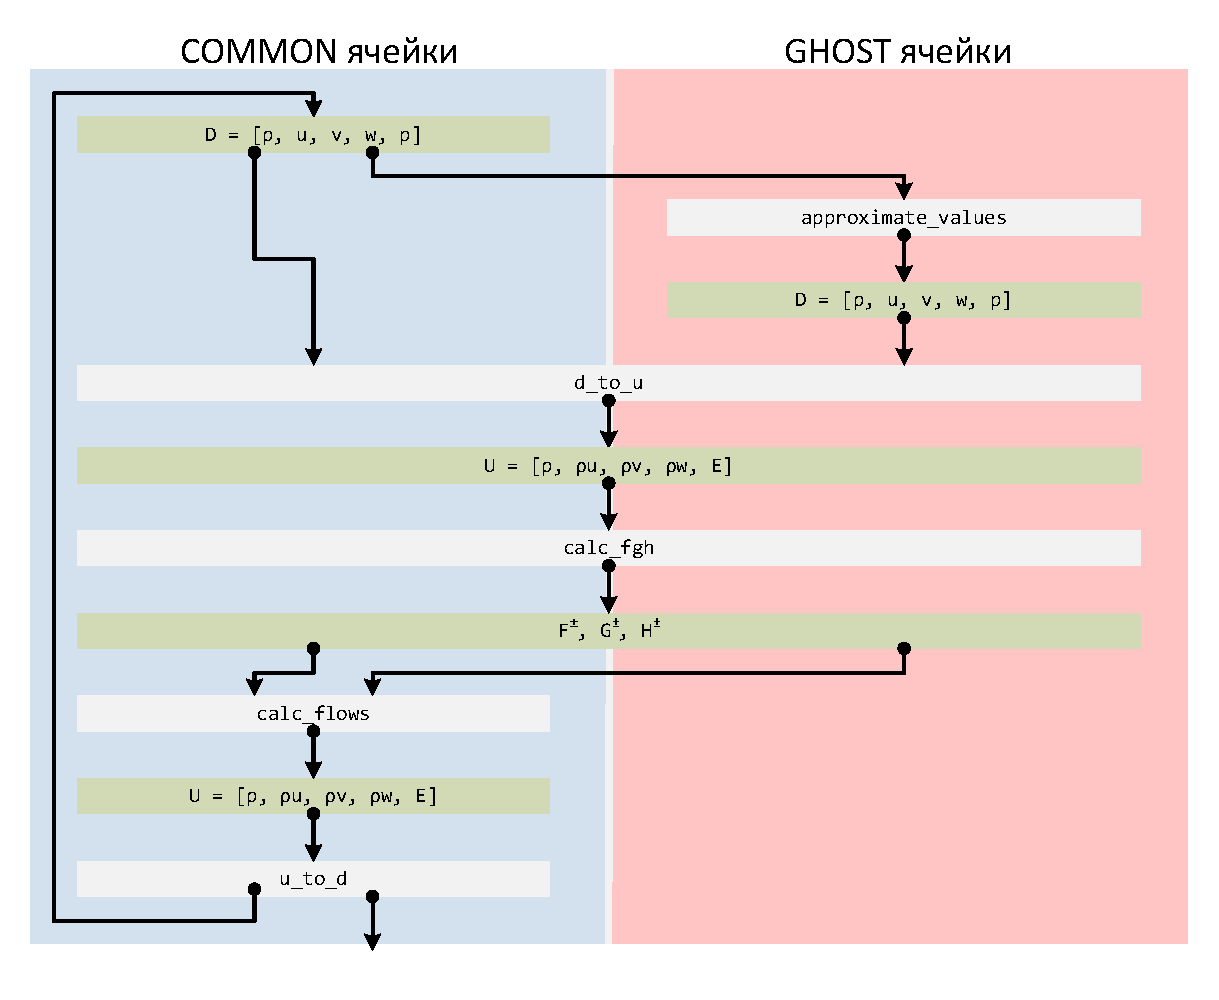
\includegraphics[width=0.8\textwidth]{./pics/text_4_ibm/immersed_boundary_method_scheme.pdf}
\singlespacing
\captionstyle{center}\caption{Схема выполнения шага расчетов методом погруженных границ с использованием схемы Стегера-Уорминга.}
\label{fig:text_4_ibm_immersed_boundary_method_cheme}
\end{figure}

Использование метода погруженных границ с фиктивными ячейками позволяет проводить газодинамические расчеты вблизи сложных границ без необходимости построения согласованных сеток.
С помощью описанного метода и с применением схемы расчета Стегера-Уорминга были проведены расчеты модельной задачи обтекания свободным потоком множества случайных сфер (при этом граница обтекаемых объектов задавалась аналитически, а не с помощью поверхностной сетки).
Во время расчетов геометрическая конфигурация оставалась неизменной, что сделало возможным однократное вычисление вспомогательных объектов для аппроксимации газодинамических величин в фиктивных ячейках (в том числе речь идет о матрицах $B_{G123}^{-1}$ и $B_{0'123}^{-1}$ из \eqref{eqn:text_1_ibm_B} и \eqref{eqn:text_1_ibm_B1}).
С помощью метода погруженных границ на декартовой расчетной сетке можно получить качественно правильную картину обтекания, что проиллюстрировано на рис.~\ref{fig:text_4_ibm_res}.

\begin{figure}[ht]
\centering
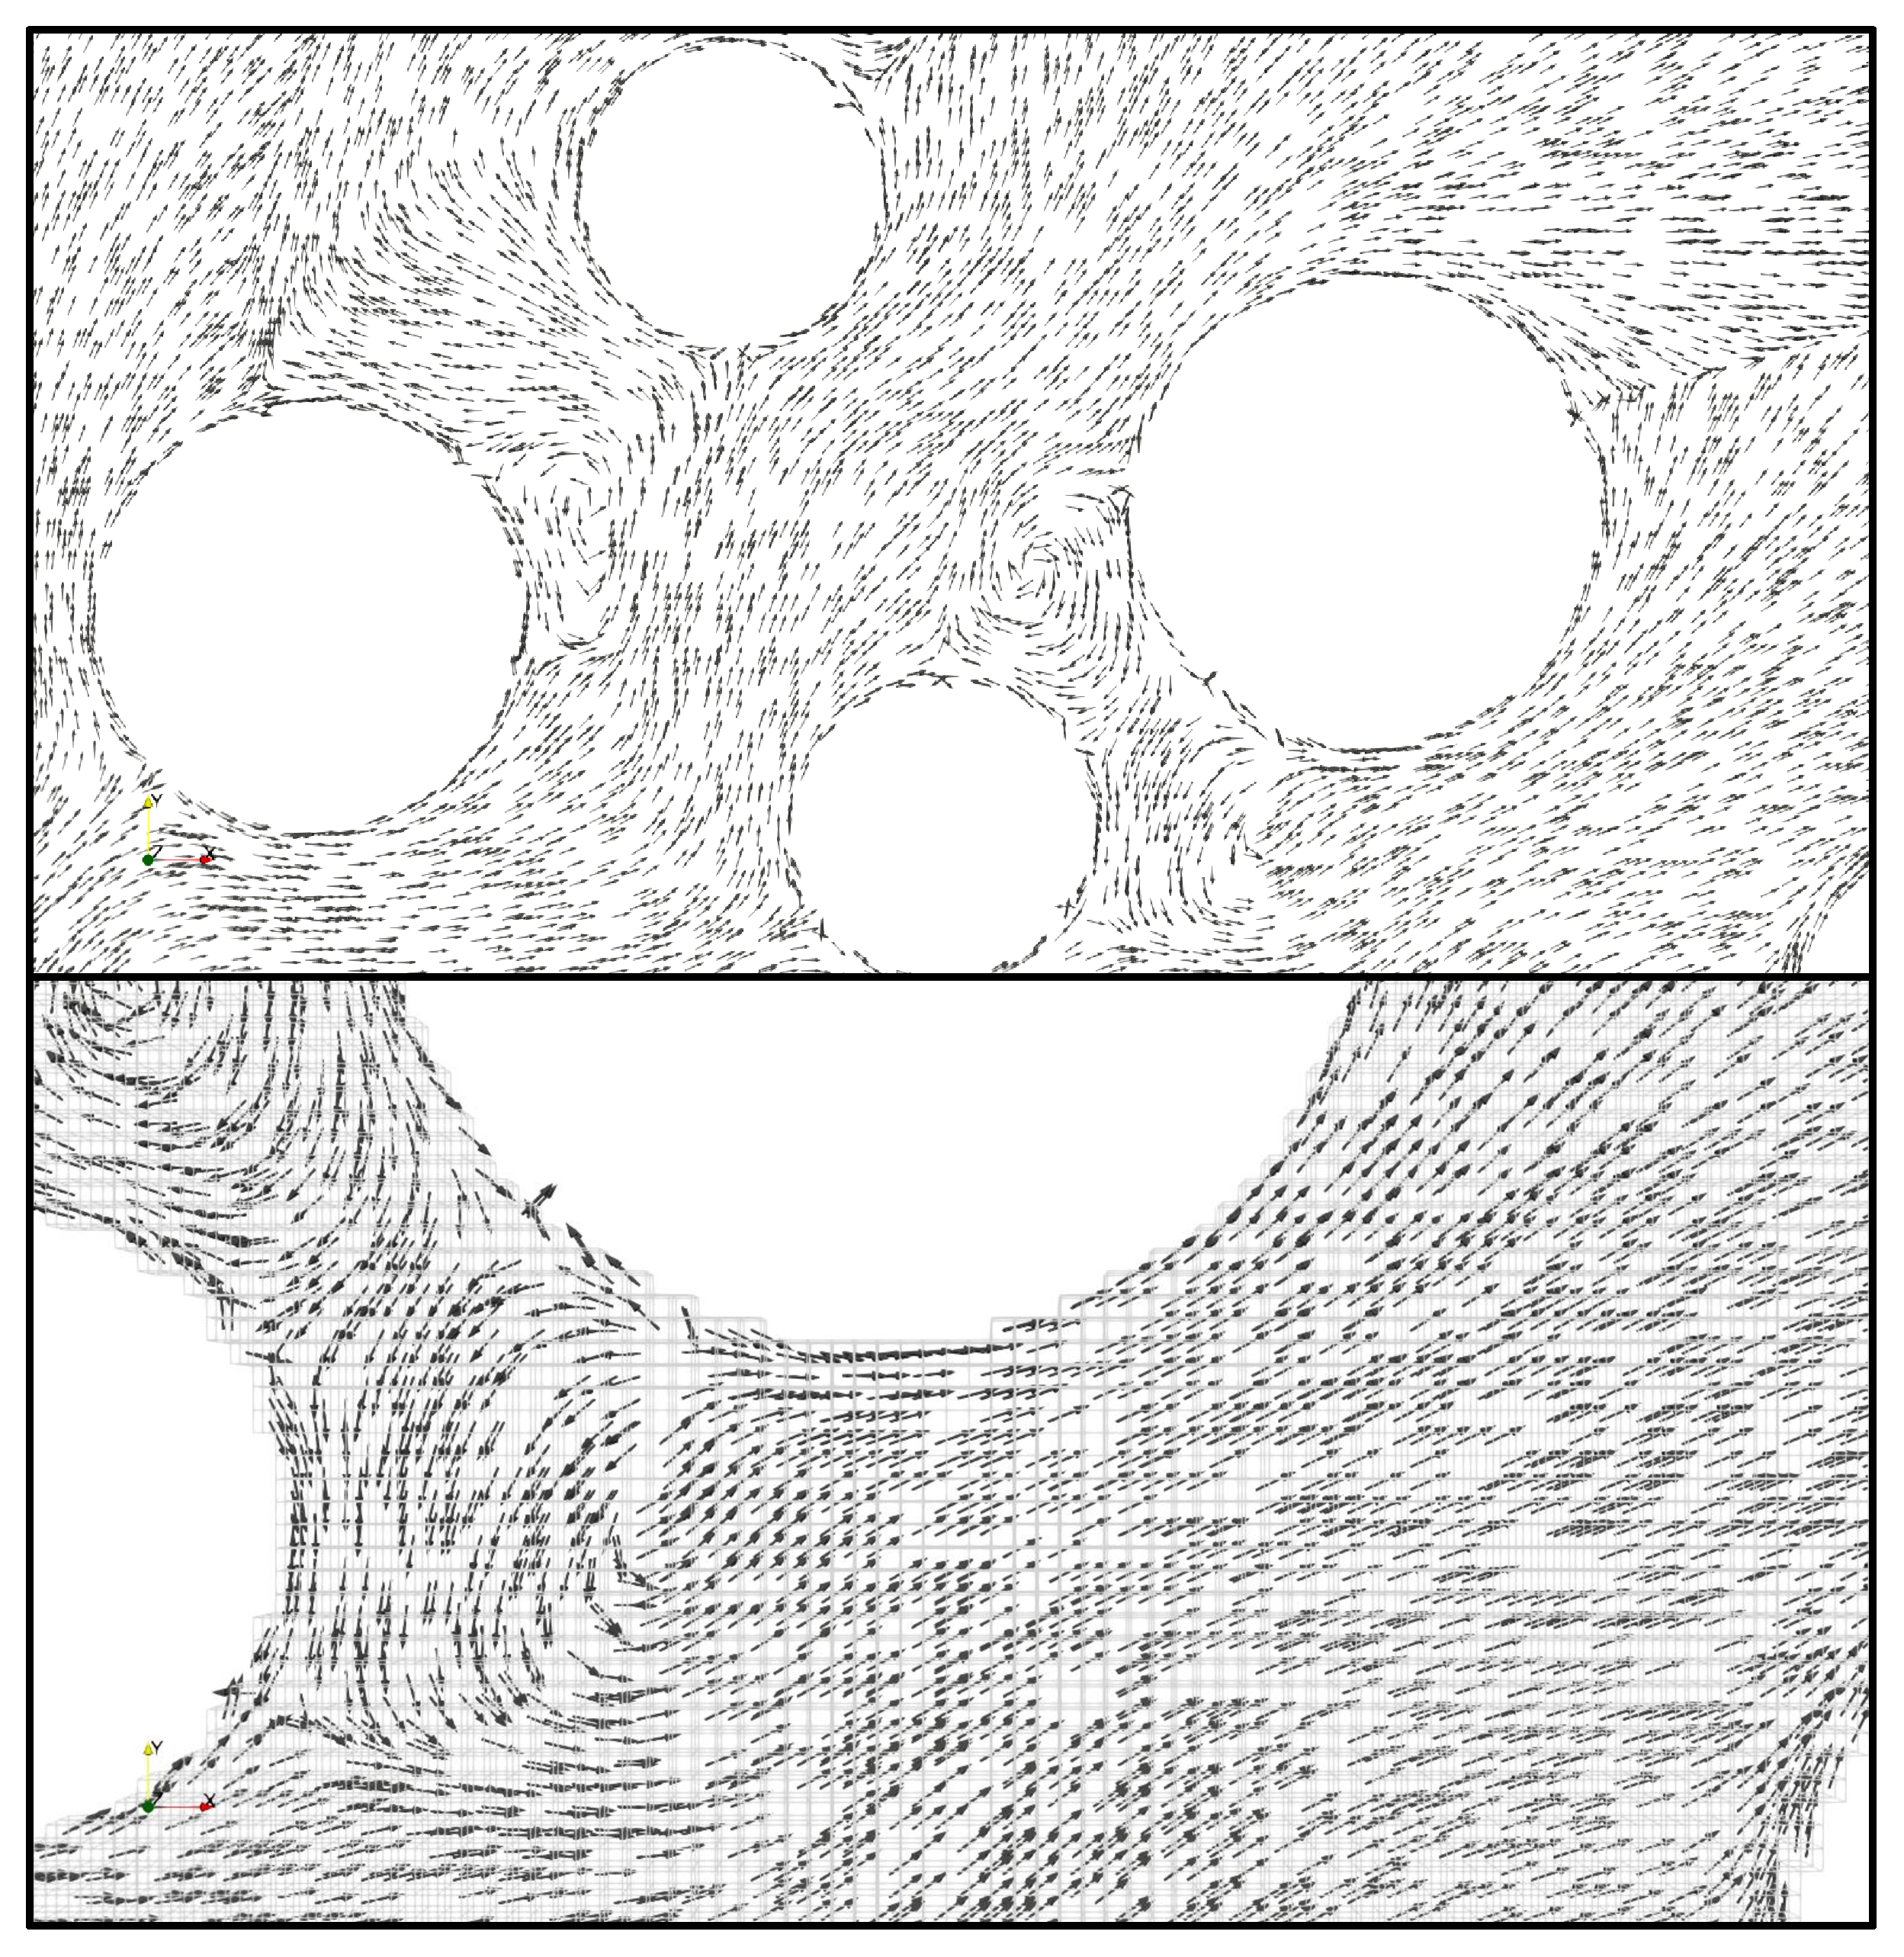
\includegraphics[width=0.8\textwidth]{./pics/text_4_ibm/res.pdf}
\singlespacing
\captionstyle{center}\caption{Визуализация поля скоростей (двумерный срез), полученного с помощью метода погруженной границы.}
\label{fig:text_4_ibm_res}
\end{figure}

Для анализа эффективности векторизации проводился эксперимент по организации программного кода газодинамического решателя, работающего с данными в формате double (вещественные числа размера 64 бита) с целью векторизации под микропроцессоры Intel Xeon Phi Knights Landing.
Этот микропроцессор был выбран, так как кроме обычных векторных арифметических операций набора AVX-512F он поддерживает также такие полезные наборы, как AVX-512PF -- операции предварительной подкачки данных из памяти и AVX-512ER -- векторные команды для вычисления экспоненты и обратных значений, которые крайне полезны в физических приложениях.

\subsubsection{Схемы организации данных <<массив структур>> и <<набор массивов>>}

Рассмотрим на примере реализации функции \texttt{d\_to\_u} из общей схемы вычислений, представленной на рис.~\ref{fig:text_4_ibm_immersed_boundary_method_cheme}, способы организации вычислений.
Итак, функция \texttt{d\_to\_u} переводит вектор примитивных газодинамических величин $D$ в вектор консервативных величин $U$ для каждой расчетной ячейки.
Интуитивным способом вычисления могут быть организованы в виде следующей схемы: для каждой ячейки создается структура, которая содержит все необходимые величины, и действия по переводу вектора $D$ в вектор $U$ выполняется над полями данной структуры (листинг~\ref{lst:text_4_vec_ibm_list_of_struct}).

\begin{lstlisting}[caption={Организация данных в виде <<массив структур>>.},label={lst:text_4_vec_ibm_list_of_struct}]
struct Cell
{
    double rho;
    double u; double v; double w;
    double p;
    double rho_u; double rho_v; double rho_w;
    double E;
};
Cell cells[N];

void d_to_u()
{
    for (int i = 0; i < N; i++)
    {
        double rho = cells[i].rho;
        double u = cells[i].u;
        double v = cells[i].v;
        double w = cells[i].w;
        double p = cells[i].p;

        cells[i].rho_u = rho * u;
        cells[i].rho_v = rho * v;
        cells[i].rho_w = rho * w;
        cells[i].E = 0.5 * rho * (u * u + v * v + w * w)
                     + p / (GAMMA - 1.0);
    }
}
\end{lstlisting}

При попытке векторизации цикла из листинга~\ref{lst:text_4_vec_ibm_list_of_struct} во время объединения нескольких последовательных итераций (объединяться должны 8 итераций, так как размер элемента данных равен 64 бита, а длина векторного регистра равна 512 бит) вместо чтения из памяти скалярного значения (например, плотности), должно происходить чтение значений плотности из несколько последовательно расположенных структур данных.
То есть чтение вектора должно осуществляться не из последовательной области памяти.
Для таких целей в наборе векторных инструкций AVX-512 предусмотрены инструкции gather/scatter, однако их эффективность гораздо ниже чтения последовательной области памяти размера 512 бит даже при использовании предварительной подкачки данных.

Естественным решением оптимизации вычислений является организация расположения данных в памяти в виде набора массивов (листинг~\ref{lst:text_4_vec_ibm_set_of_lists}).
Теперь после объединения нескольких итераций цикла команды скалярного доступа в память трансформируются в векторные аналоги доступа к последовательной области памяти размера 512 бит.
Вся же арифметика, которая присутствует в коде функции (операции сложения, вычитания, умножения, деления, взятие обратной величины) имеет свои векторные аналоги в наборе инструкций AVX-512.

\begin{lstlisting}[caption={Организация данных в виде <<набор массивов>>.},label={lst:text_4_vec_ibm_set_of_lists}]
double rhos[N];
double us[N]; double vs[N]; double ws[N];
double ps[N];
double rho_us[N]; double rho_vs[N]; double rho_ws[N];
double Es[N];

void d_to_u()
{
    for (int i = 0; i < N; i++)
    {
        double rho = rhos[i];
        double u = us[i];
        double v = vs[i];
        double w = ws[i];
        double p = ps[i];

        rho_us[i] = rho * u;
        rho_vs[i] = rho * v;
        rho_ws[i] = rho * w;
        Es[i] = 0.5 * rho * (u * u + v * v + w * w)
                + p / (GAMMA - 1.0);
     }
}
\end{lstlisting}

\subsubsection{Расщепеление циклов по условию для сокращения количества условий}

Другой критической проблемой, влияющей на эффективность векторизации кода, является наличие условных операций внутри векторизуемого плоского цикла.
Конечно набор инструкций AVX-512 содержит специальные масочные аргументы, с помощью которых можно векторизовать программный код с управлением практически любой сложности (разветвленное управление, гнезда циклов, циклы с вызовами функций, циклы с нерегулярным числом итераций), однако при увеличении количества условий в коде эффективность векторизации снижается.

В качестве примера такого негативного эффекта можно рассмотреть логику гнезда циклов из функции \texttt{calc\_flows}, в которой корректируются консервативные величины с помощью потоков через все грани ячейки.
Пусть рассматриваемая расчетная область представлена структурированной сеткой размера $NX \times NY \times NZ$ по направлениям $i$, $j$, $k$ соответственно.
Тогда при учете потоков через левую грань каждой ячейки необходимо отдельно обрабатывать случай $i = 0$, что соответствует граничному условию расчетной области, причем это граничное условие может быть разных видов (свободное протекание, условие жесткой стенки) (см. листинг~\ref{lst:text_4_vec_ibm_nest}).
Аналогично нужно рассматривать особые случаи для всех шести граней ячейки, что резко увеличивает количество условий внутри цикла и снижает эффективность векторизации.

\begin{lstlisting}[caption={Гнездо циклов с условием во внутреннем цикле.},label={lst:text_4_vec_ibm_nest}]
for (int k = 0; k < NZ; k++)
{
    for (int j = 0; j < NY; j++)
    {
        for (int i = 0; i < NX; i++)
        {
            if (i == 0)
            {
                // left boundary condition
                ...
            }

            // rest code
            ...
        }
    }
}
\end{lstlisting}

\begin{lstlisting}[caption={Расщепление гнезда циклов по условию.},label={lst:text_4_vec_split_nest}]
for (int k = 0; k < NZ; k++)
{
    for (int j = 0; j < NY; j++)
    {
        // left boundary condition with i = 0
        ...
    }
}

for (int k = 0; k < NZ; k++)
{
    for (int j = 0; j < NY; j++)
    {
        for (int i = 1; i < NX; i++)
        {
            // rest code
            ...
        }
    }
}
\end{lstlisting}

Можно заметить, что условия обработки границ расчетной области не являются уникальными для тройки координат ячейки $(i, j, k)$, но являются константными для некоторого среза ячеек сетки.
Это означает, что для гнезда циклов такое условие является частично константным, и гнездо может быть разбито по этому условию.
На листинге~\ref{lst:text_4_vec_split_nest} продемонстрировано разбиение гнезда циклов по условию $i = 0$, после чего итоговое гнездо, содержащее основную часть вычислений, освобождается от условия.
Аналогичным образом можно выполнить разбиение по остальным условиям, освободив от них основное гнездо циклов, которое после этого успешно векторизуется.

На рис~\ref{fig:text_4_ibm_immersed_boundary_method_cheme} представлена общая схема выполнения расчетов для одной итерации численного метода.
Основными функциями в этих расчетах являются \texttt{approximate\_values}, \texttt{d\_to\_u}, \texttt{calc\_fgh}, \texttt{calc\_flows}, \texttt{u\_to\_d}.
Во время проведения эксперимента на модельной задаче был собран профиль исполнения до векторизации и после нее, результаты распределения времени исполнения между этими основными функциями представлены на рис.~\ref{fig:text_4_ibm_diagr}.

\begin{figure}[ht]
\centering
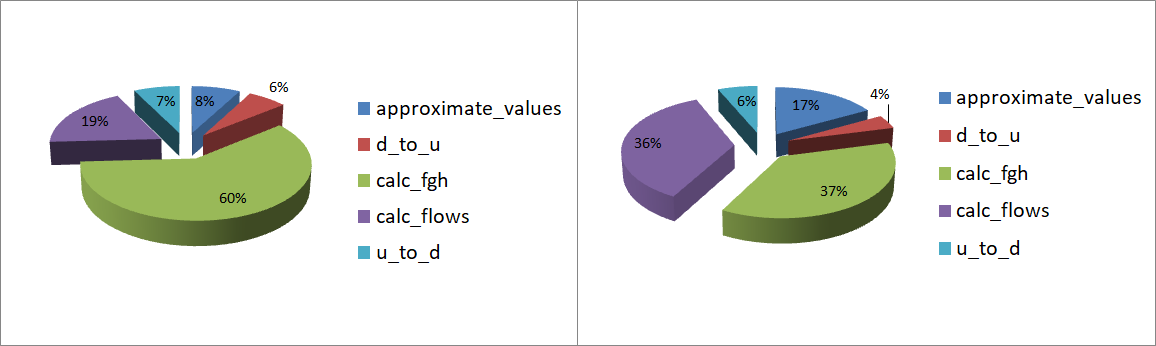
\includegraphics[width=1.0\textwidth]{./pics/text_4_ibm/diagr.png}
\singlespacing
\captionstyle{center}\caption{Распределение времени выполнения отдельных функций газодинамического решателя.}
\label{fig:text_4_ibm_diagr}
\end{figure}

Также на рис.~\ref{fig:text_4_ibm_diagr2} представлены результаты ускорения после векторизации каждой функции в отдельности и суммарного ускорения всего расчетного кода.
Заметим, что во время векторизации расчетного кода, работающего с вещественными числами двойной точности, один векторный регистр содержит 8 элементов данных.
На практике ускорение в 4 раза для расчетных кодов, работающих с числами формата double, в результате векторизации уже можно считать успешным.

\begin{figure}[ht]
\centering
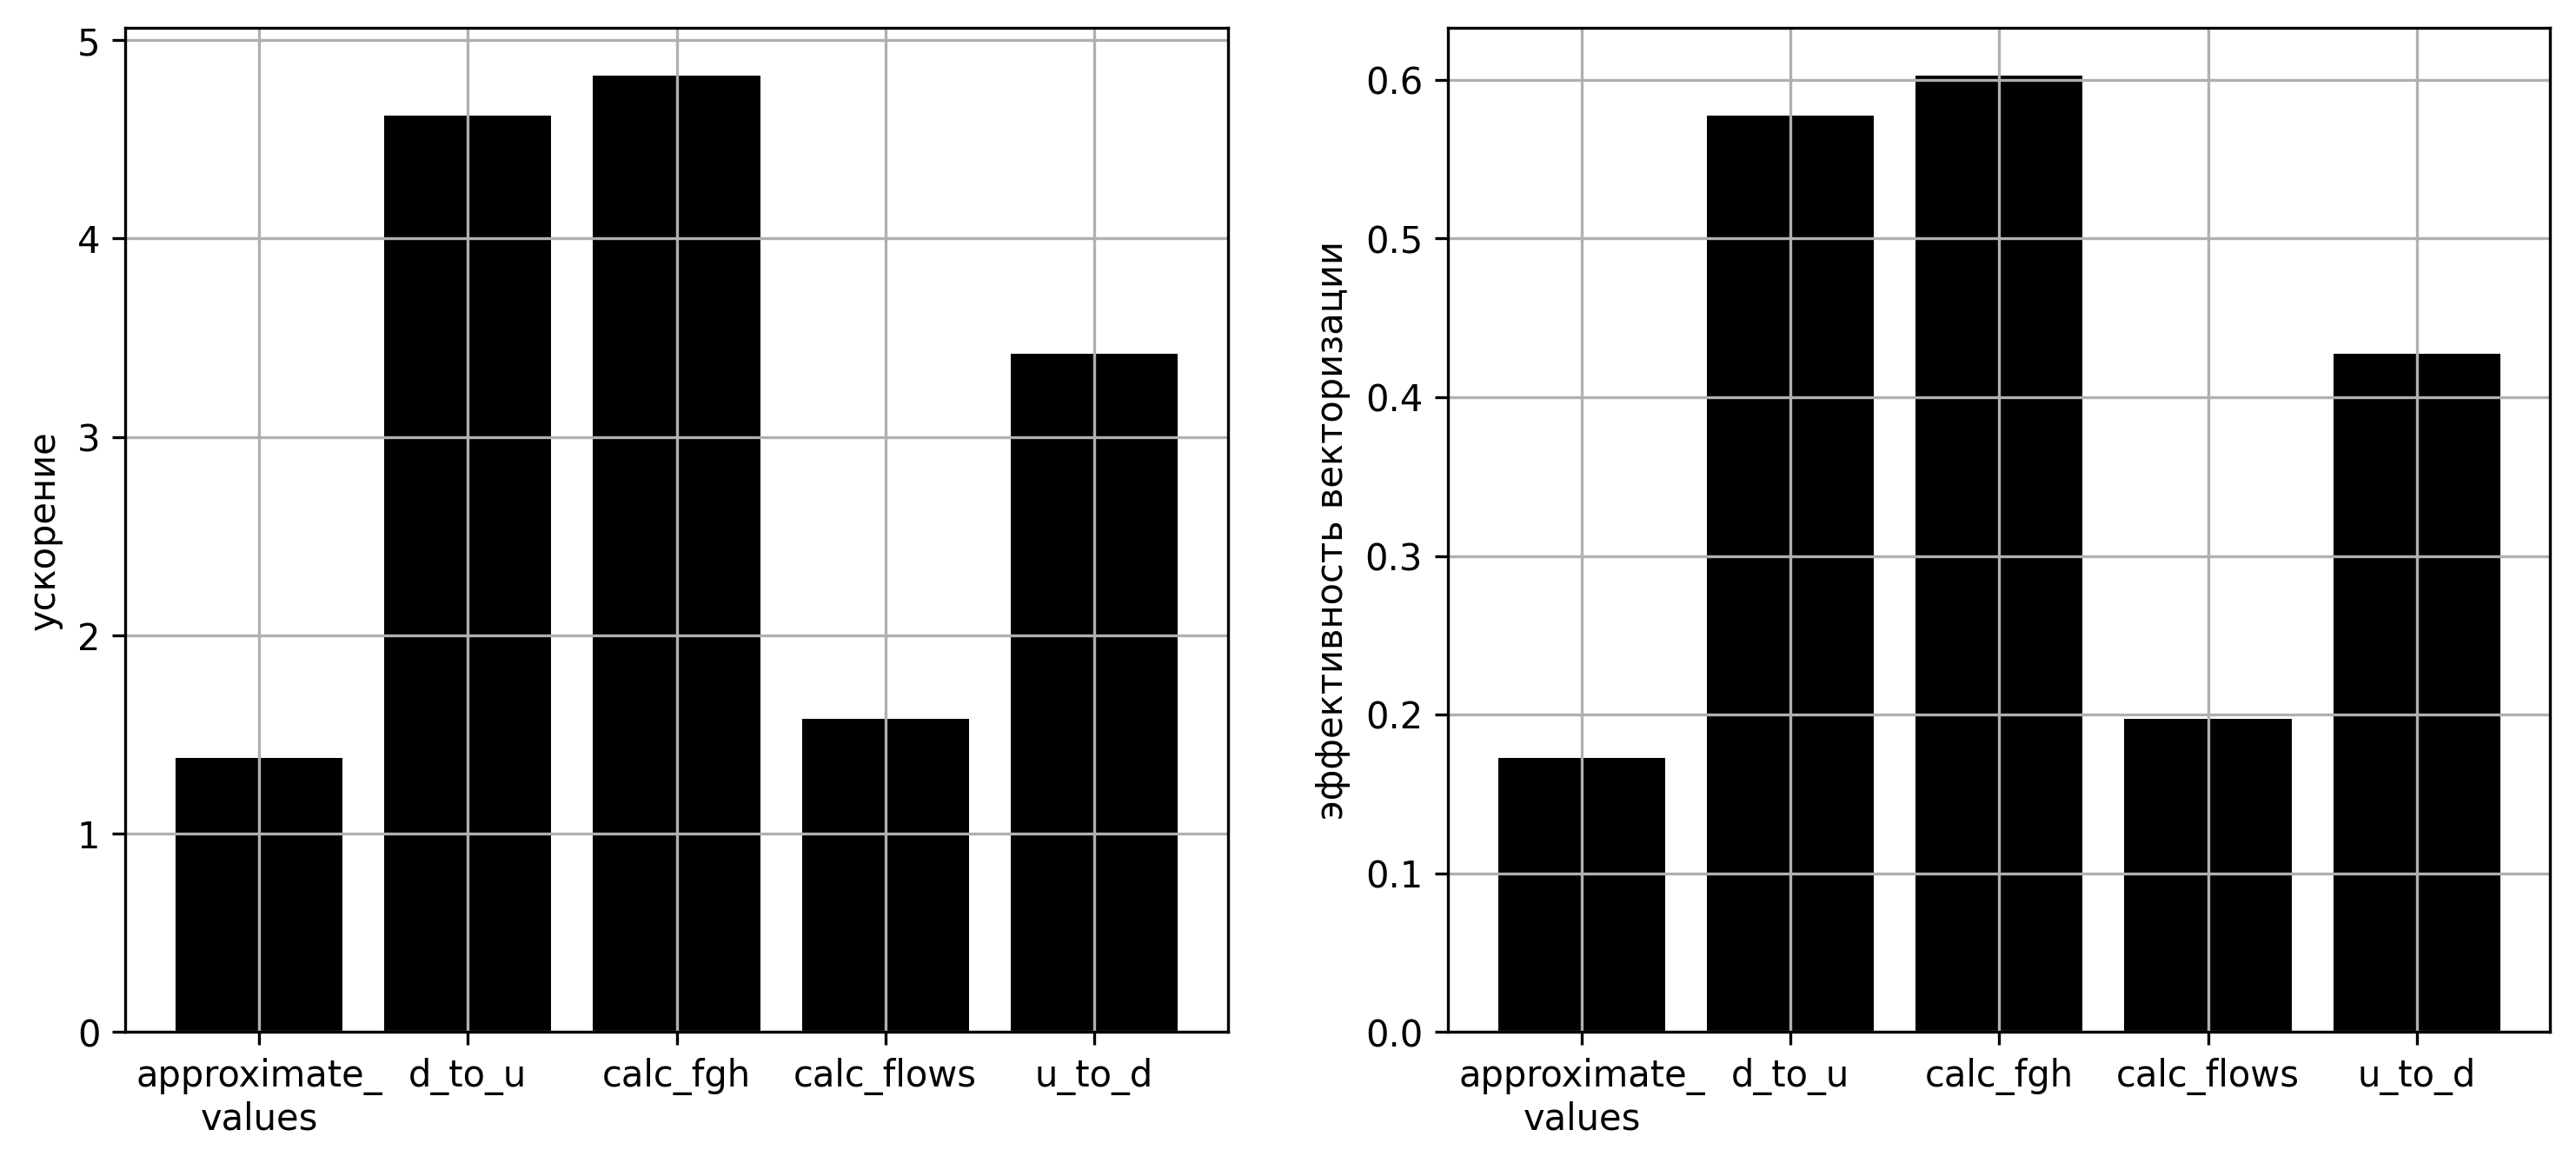
\includegraphics[width=1.0\textwidth]{./pics/text_4_ibm/diagr2.png}
\singlespacing
\captionstyle{center}\caption{Эффективность векторизации отдельных функций газодинамического решателя.}
\label{fig:text_4_ibm_diagr2}
\end{figure}

Заметим, что ускорение различных функций в результате векторизации сильно отличается друг от друга.
Причиной этому являются конкретные особенности каждой из этих функций.

Наибольшее ускорение продемонстрировала функция \texttt{calc\_fgh}, реализующая вычисление потоков $F^{\pm}$, $G^{\pm}$, $H^{\pm}$.
Этому способствовали следующие особенности этой функции.
Во-первых, функция содержит плоский цикл, полностью удовлетворяющий всем условиям, что делает возможным замену всех скалярных операций на векторные аналоги.
Во-вторых, в скалярной версии используются библиотечные вызовы \texttt{abs} (вычисление абсолютного значения) и \texttt{sqrt} (вычисление квадратного корня).
В наборе векторных инструкций AVX-512 есть векторные операции VAND (с помощью побитовой операцией над вещественным числом можно обратить в ноль бит знака данного числа), VSQRT, которые реализуют эти действия просто одной операцией, что сильно ускоряет исполнение.
Наконец, обилие операций умножения и сложения делает возможным применение векторных комбинированных операций вида $\pm a \cdot b \pm c$.

Также ускорение выше среднего продемонстрировали функции \texttt{d\_to\_u} и \texttt{u\_to\_d}.
Эти функции также состоят из плоских циклов, поэтому скалярные операции могут быть заменены на векторные аналоги.
Более низкое ускорение функции \texttt{u\_to\_d} объясняется наличием операций деления, которые выполняются медленнее операций сложения и умножения.

Показатель ускорения функции \texttt{calc\_flows} составил менее двух раз даже после избавления от всех условий, связанных с обработкой границ расчетной области.
Такая низкая эффективность векторизации объясняется тем, что внутри этой функции присутствуют циклы, которые не являются плоскими.
Так, например, в функции \texttt{calc\_flows} для корректировки консервативных величин внутри ячейки $(i, j, k)$ требуется обращаться за данными ко всем смежным по граням ячейкам: $(i \pm 1, j, k)$, $(i, j \pm 1, k)$, $(i, j, k \pm 1)$.
Это нарушает требование по унификации обращения к массивам данных на одной итерации плоского цикла и немедленно приводит к появлению операций gather/scatter, понижая эффективность векторизации.
Для функции \texttt{approximate\_values} ситуация выглядит аналогичной, так как для выполнения аппроксимации данных в ячейке $(i, j, k)$ требуется обращаться за данными в ячейки, относящиеся к шаблону аппроксимации (на рис~\ref{fig:text_4_ibm_immersed_boundary_method_cheme} нарушение требования унификации обращения за данными продемонстрировано красными стрелками, означающими, что при обработке одной ячейки сетки мы вынуждены обращаться за данными к другой ячейке).

Несмотря на низкие показатели эффективности векторизации функций, содержащих циклы, не являющиеся плоскими, общая эффективность от векторизации метода погруженных границ составила примерно три раза, при этом удалось ограничиться только реорганизацией кода без использования ассемблера или функций-интринсиков для форсированного использования векторных инструкций.
